\chapter{Fisher's Linear Discriminant}
\label{ch:chapter2}
 
The main objective of this chapter is to introduce the Fisher's Linear Discriminant Analisis (FLDA), which looks to optimize the trace $\Tr(V^T A V) / \Tr(V^T B V)$ over the set of ortogonal matrices $V$ with $A, B$ positive definite matrices. To give a solution to the problem, different formulations of the problem have been given in statistical learning and pattern recognition books, but because of the computational cost, \cite{wang2007trace} \cite{ngo2012trace} the original had not a solution. Different reformulation of the problem as: maximize the trace of the between-scatter matrix with a restriction over the within-scatte matrix; or another one was to maximze the ratio of determinants or to maximize the trace of the ratio of these matrices have been formuled. \cite{duda2012pattern} \cite{hastie2009elements} \cite{mitchell2006discipline} \cite{fukunaga2013introduction}. At the end, all these formulations are simplified objective functions of the original one.

In this chapter a efficient solution for the FLDA trough the Newton-Lanczos method will be given. In the first section, the problem will introduced as a problem of Machine Learning. In the second, the theory will be given to follow easily the text. In the third section, an intuitive solution for the problem in the case of one dimension projectors will be presented and then it will be generalized to $p$ dimensions. At last, the necessary and sufficient conditions for the optimization problem will be derived.


\section{Machine Learning}
 
Machine learning is founded in two research areas: Computer Sciences and Statistics. From the first, it takes the questions: How can we build machines that solves problems? and, Given the actual techonology, What kind of problems are feasibles to solve? On the other hand, from Statistics it tryes to answer: What conclusions can be infered from the dataset? and How can we manage the uncertainty of this method? \cite{mitchell2006discipline}. The joint work from both areas to try to answer these questions helps to build a computational statistical framework of machine learning.

\section{The learning process}

A machine \textit{learns} given a task (T), a measure of the performance (R) and a type of experience (E) if the system improves the performance (R) in the task (T) with this expericence (E) \cite{mitchell2006discipline}. With the data, we try to model a structure in order that the machine improves their performance when it receives more information. The diversity of the task, as well as the applications is big. For example:

\begin{itemize} 

\item \textit{Spam/no-spam classification}, Here, (E) are the emails, (T) the task to classify correctly the \textit{spam} y (R) the proportion of correctly classified emails.

\item \textit{Face recognition/classification}, Here, (E) are the faces of distinct people, (T) is the correct classification of the faces and (R) is the measured as the percentage of correct classified faced.

\end{itemize} 

The learning proceses have many applications and distinct assumptions. For this reason, is useful to provide a framework that groups all the methods given some criteria. The classification used here is the proposed for T. Hastie \cite{hastie2009elements}. This divides the methods in two groups: Supervised learning and unsupervised learning. The first assumes the an output variable that helps to build the structure of the model. Examples of this are the Linear Regression, the decission and classification trees (CART) and the Support Vector Machines (SVM). On the other hand, the unsupervised learning only uses the information of the independent variables. For example, cluster análisis, asociation rules and some dimensiontality reduccion methods.

After this first classification, a subgroups are of the supervised methods are made depending of the output variable \footnote{In this text will be used the terms input variable and ouput variables as the  dependant and independant variables respectively} When the model considers a quantitative variable, then it recives the name of regression, and when it is a categrical variable it receives the name of classification. On the other hand, the unsupervised learning have two main branches \cite{hastie2009elements}. The first is called segmentation, in which each individual is assigned to one group in a way that inside the group they are homogeneus between them, but between groups they are different. The second group of methods is the dimensitonality reduction, in which we try to project the individuals of the dataset into a much subspace of the space generated from the original dataset.

The Fisher's LDA is a subbranch of the supervised learning, in particular of the classification methods. Alternative linear methods for this, is the Logistic Regresion, the Classic Linear Discriminant Analysis and the Support Vector Machines.


\section{Dispersion matrices}
First of all, the nomenclature will be defined. $\mathbb{C} = {k; k = 1, 2, 3, ..., K}$ will be the set of the $K$ distinct classes where the each observation $x_i$ with $i = 1, ..., N$ can be assigned and $N$ the total number of observation. Then let's define as $C_k$ the subset of the ${1, 2, 3, ..., N}$ observations where each one of these is part of the set $C_k$ that contains the indices of the observations belonging to the class $k$. This way, let's define as $N_{k}$ to the number of observations in class $k$. At last $w_i = V^T x_i$ is the data multiplied with the matrix $V$, or equivalentely, the projected observation. Then, the means of each group $k$ are $\mu_k$ and the global mean of all the observation is defined as $\mu$:

\begin{equation} \label{eq:18}
  \mu_k = \frac{1}{N_{k}} 
  \sum_{i  \in C_k}
                  x_i
\end{equation} 

\begin{equation} \label{eq:19}
 \mu = \frac{1}{N} \sum_{i = 1}^{N} x_i
\end{equation}

On the other hand, let's define the mean of the projected observations $w_i$:
\begin{equation} \label{eq:20}
  \widetilde{\mu_k} = \frac{1}{N_{k}} 
  \sum_{i \in C_k}
                  w_i
\end{equation} 

\begin{equation} \label{eq:21}
 \widetilde{\mu} = \frac{1}{N} \sum_{i = 1}^{N} w_i
\end{equation}

The Fisher's Linear Discriminant Analysis uses in its computation the dispersion matrices. In specific, the covariance matriz, the scatter matrix of all the observations, the intra-class scatter and the between class scatter. It is important to analize the terminology and the formulas that will be used in this thesis in order to undestand the logic behind the formulation of the optimization problem.

$\Sigma$ will represent the covariance matrix of all the observations. Let's define as $\widehat{\Sigma}$ to the unbiased estimator of $\Sigma$ which is divided by $N-1$:

\begin{equation} \label{eq:2.1}
\widehat{\Sigma} = \frac{1}{N-1} \sum_{i=1}^{N}(x_i - \mu)(x_i - \mu)^T	
\end{equation}

If this matrix is not scaled by the $N-1$ factor, then it is know as Scatter matrix. In this tesis, is represented as $S_T$, with the subindex $T$ meaning that is taking all the observations for this computation

\begin{equation} \label{eq:2.2}
S_T = \sum_{i=1}^{N}(x_i - \mu)(x_i - \mu)^T	
\end{equation}

If the matrix is only considering all the observacions that belongs to the class $k$, this will be represented as $S_k$, with the subindex $k$ meaning that it is taking the scatter of just the observations with class $k$:

\begin{equation*}
S_k = \sum_{i=1 \in C_k} (x_i - \mu)(x_i - \mu)^T	
\end{equation*}

The same way we are going to define the Within-class scatter matrix, as the sum over all the $k$ scatter matrix presented above.

\begin{equation}\label{eq:2.3}
S_I = \sum_{k=1}^{K} 
					\sum_{i \in C_k}
 ({x_i-\mu_{k}})({x_i-\mu_{k}})^T 	
\end{equation}

Now, let's define the Between-class scatter matrix as the sum of all the squared differences of the mean of each class with respect to the global mean of all the observations. This is multiplied by the number of observations in each class $k$ ($N_k$).

\begin{equation} \label{eq:2.4}
S_E = \sum_{k = 1}^K N_k (\mu_k - \mu)(\mu_k - \mu)^T	
\end{equation}

\begin{figure}[!ht] \label{Fig1.1}
  \centering
	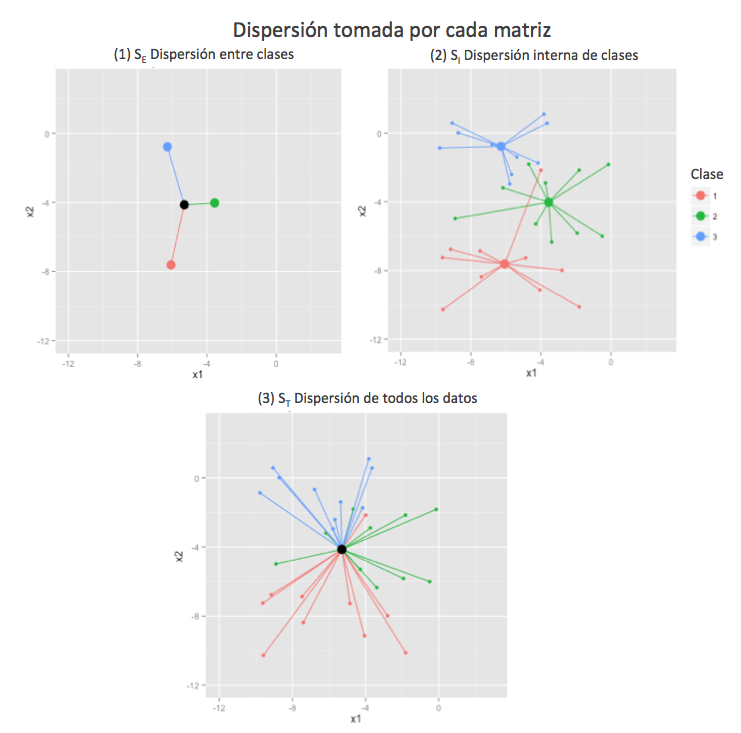
\includegraphics[width=1\textwidth]{Figures/Chapter2_SE_SI}	
  \caption[Distances considered in each scatter matrix.]
  {In the plot (1) it is represented the distances between the mean of all the observations (black points) and the means of each class (color points). The plot (2) represents $S_I$: the squared difference between each observation and the mean of all the observations that are in the same class. Finally, in the plot (3), it is represented $S_T$, the scatter of all the data with with respect to the global mean}
\end{figure}

Between the Within-class scatter matrix $S_I$, the Between-class scatter matrix and the total scatter matrix there is an important relationship. It is always true that $S_T = S_I + S_E$; then, 
if we add the information for each class to the observations, then the total scatter matrix can be factorized as the sum of the Within-class scatter matrix and the Between-class scatter matrix.

\pagebreak
As an example of the relation $S_T = S_I + S_E$, 10 normally distributed observations were generated for each class. (The correlation coefficient for the generated data is $-0.005$). Then, calculating the scatter matrices from the formulas (1.6), (1.7) and (1.8), we have the following equivalences: 
\begin{center}
\begin{tabular}{ c c c}
\toprule
\textbf{Clase} & \textbf{Distribución x1} & \textbf{Distribución x2} \\
\midrule\\
\addlinespace[-2ex]
1 & N(-5, 2.5) & N(-8, 2)\\
2 & N(-3, 2.5) & N(-4, 2)\\
3 & N(-7, 2.5) & N(-1, 2) \\
\addlinespace[1.5ex]
\bottomrule
\end{tabular}
\end{center}

\begin{center}
\begin{tabular}{ c c c}
\toprule
\textbf{$S_I$} & \textbf{$S_E$} & \textbf{$S_T$} \\
\midrule\\
\addlinespace[-2ex]
$ \begin{bmatrix}  186.05 & 2.78 \\ 2.78 &  94.58 \end{bmatrix}$ &
$ \begin{bmatrix} 46.13 & -4.15 \\ -4.15 & 234.57 \end{bmatrix}$ &
$ \begin{bmatrix}  232.18 & -1.36 \\ -1.36 &  329.16 \end{bmatrix}$ \\
\addlinespace[1.5ex]
\bottomrule
\end{tabular}
\end{center}

This is important because, as seen in the next chapter, the proposed problem can be rewritten just with the total scatter matrix in the numerator ot the trace ratio instead of the between-scatter matrix. Now, a very common problem that arises in machine learning problems is that the cost of the computation can become intractable with the dimensionality of the observations increases. In the Fisher's Linear Discriminana Analysis it is required that the scatter matrices of the observations be recomputed in each iteration and also, to calculate the inverse or pseudoinverse of a matrix. These steps can become quite expensive. As a solution to the problem of dimensionality (or commonly named curse of dimensionality) here we propose to use the Principal Component Analysis as prior step to reduce the dimensionality of the original data. This method is very easy to calculate and te standard linear algebra libraries are optimized to do this \cite{ngo2012trace}. Due to the objective of this thesis no more techniques will be considered for the dimensionality reduction, but books as \cite{hastie2009elements} and \cite{duda2012pattern} propose distinct methods to solve this problem.

Now, coming back to the original problem, we want to find the projection that keep togueters the observations that belong to the same class, at the same time that the centroid of each class is far. When this projection is obtained, then is easy to find an hyperplane that separates the different classes.

\pagebreak
The optimization problem can be formulated as:
\begin{equation}\label{eq:2.5}
	\max_{\substack{V \in {\rm I\!R}^{n \times p} \\ V^TV = I}} \frac{\Tr(V^T S_E V)}{\Tr(V^T S_I V)}
\end{equation}

The solution for this problem does not have a closed form, so in the literature distinct formulations have arised to solve it analytically \cite{wang2007trace} \cite{fukunaga2013introduction}. Some of these formulations are listed below: 

\begin{equation}\label{eq:2.6}
	\max_{\substack{V \in {\rm I\!R}^{n \times p} \\ V^T S_I V = I}} \Tr(V^T S_E V)
\end{equation}

\begin{equation} \label{eq:2.7}
	\max_{\substack{V \in {\rm I\!R}^{n \times p} \\ V^T V = I}} \Tr\left( \frac{V^T S_E V}{V^T S_I V}\right) 	
\end{equation}

\begin{equation} \label{eq:2.8}
	\max_{\substack{V \in {\rm I\!R}^{n \times p} \\ V^T V = I}} \frac{|V^T S_E V|}{|V^T S_I V|} 	
\end{equation}

with $|\bullet| = det(\bullet)$ y $\Tr(\bullet) = Trace(\bullet)$.

In the next part of this chapter, the original problem (1.9) will be solved when $p = 1$, and for this reason, the generalized Rayleigh quotient is introduced. For the generalization to $p$ dimensions only the problem will be formulated and then the existence and uniqueness will be determined. Afterwards, a new function $f(\rho)$ will be defined. This is useful because is easier to work numerically with this function instead of working with the original trace ratio. At last, using the eigenvalues of $S_I$ y $S_E$ the optimal value $\rho^*$ will be bounded.

\section{Trace ratio problem}

In this text, when using the term projection it will always refer to the ortogonal transformation given by the matrix $V = [V_1 | V_2 | ... | V_p ]$ with $V \in {\rm I\!R}^{n \times p}$. \footnote{This matrix have ortogonal columns, then assuming that each column has norm 1, then $V^T V = I_p$} Let $X = [X_1 | X_2 | ... | X_m ]$ the matrix of observations of size ${\rm I\!R}^{n \times m}$, then when we expand $V^T X$:

\begin{equation*}
V^T X= \left(\!
    \begin{array}{cccc}
      V_1^T (X_1) &  V_1^T (X_2) & \hdots & V_1^T (X_m) \\
      V_2^T (X_1) &  V_2^T (X_2) & \hdots & V_2^T (X_m) \\
      \vdots & \vdots & \ddots & \vdots\\
      V_p^T (X_1) &  V_p^T (X_2) & \hdots & V_p^T (X_m) \\
    \end{array}
  \!\right) 
\end{equation*} 

As can be seen, each entry of the matrix $V^T X$ is equal to $V_i^T X_j$: a dot product between a colum of $V$ and a row of $X$. On the other side, we have that $\vectorproj[V_i]{X_j} = \frac{X_j \cdot V_i}{\norm{V_i}^2} V_i$. Like $\norm{V_i} = 1$, then the formula is simplified as $\vectorproj[V_i]{X_j} = (X_j \cdot V_i) V_i$; equivalently a vector of norm $(X_j \cdot V_i)$ in the direction of $V_i$. Because of this reason, this are the projected observations: each observation is projected by each column of $V$.

The trace ratio problem is easy to analize when $V \in {\rm I\!R}^{n \times p}$ projects to a lower dimensional space. For example, when $p = 2$, then the problem is equivalent to find the best projection to a plane, and when $p = 1$, to the best projection to a vector. As an example, a sintetic dataset was created, where each $x_i \in {\rm I\!R}^{3}$. In this dataset the distributions are normally distributed and are projected in${\rm I\!R}^{2}$ and ${\rm I\!R}^{1}$. These data can be observed in the figure 1.3.

\begin{figure}[!ht]\label{Fig1.2}
  \centering
  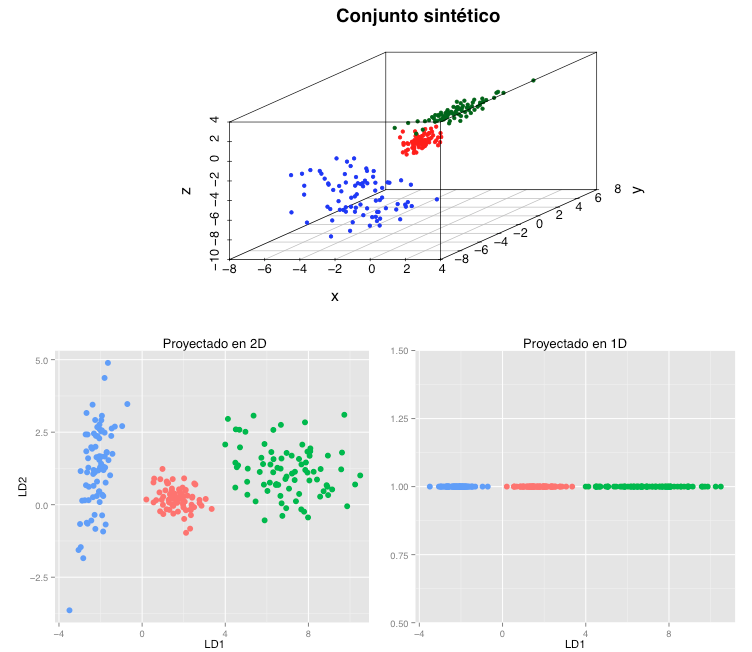
\includegraphics[width=1\textwidth]{Figures/Chapter2_1} 
  \caption[Best projections in ${\rm I\!R}^{2}$ y ${\rm I\!R}$.]
  {In the above graph it is shown the original data in ${\rm I\!R}^{3}$. In the graph in lower left  it is shown the best projection in ${\rm I\!R}^{2}$ and in the right the best projection in ${\rm I\!R}$}
\end{figure}

\subsection{Solución when p = 1}

The problem (1.9) is quite straighforward when $V \in {\rm I\!R}^{n}$. $v$ is a one dimensional projection:


\begin{equation} \label{eq:2.9}
\max_{v \in {\rm I\!R}^{n}} \frac{v^T S_E v}{v^T S_I v}  
\end{equation}

Again, $x_i \in {\rm I\!R}^{n}$ are the original observations with $i = 1 , ... , N $. Then $w_i \in {\rm I\!R}$ are the projected observations with the vector $v$. This way $w_i = v^Tx_i$. It is convinient to define $\widehat{\mu}_k = v^T \mu_k$ y $\widehat{\mu} = v^T \mu$ as the mean of the class and the mean of all the projected observations. The projected Between-class scatter matrix and the projected Within-class scatter matrix are now defined as:

\textbf{Between-class scatter matrix $\Phi_{E}$ of the projected observations $w_i$:}

$$\Phi_{E} = \sum\limits_{k =1}^{K} N_k (\widehat{\mu}_k - \widehat{\mu} )^2$$

$$\Phi_{E} = \sum\limits_{k =1}^{K} N_k (v^T \mu_k - v^T \mu)^2$$

$$\Phi_{E} =  \sum\limits_{k =1}^{K} N_k v^T ( \mu_k - \mu )(\mu_k - \mu )^T v $$
Because of the property of distributivity in for the matrix, we have that $vAv+vBv =  v(A+B)v$, then:

\begin{equation}\label{eq:2.10}
\Phi_{E} = v^T \big[ \sum\limits_{k =1}^{K} N_k ( \mu_k - \mu )(\mu_k - \mu )^T \big] v	
\end{equation}

\textbf{Intra-class scatter matrix $\Phi_{I}$ of the projected observations $w_i$}:
$$\Phi_{I} = \sum\limits_{k = 1}^{K} \sum\limits_{i \in C_k} (w_i - \widehat{\mu}_k)^2 $$
$$\Phi_{I} = \sum\limits_{k = 1}^{K} \sum\limits_{i \in C_k} (v_i^T x_i - v_i^T \mu_k)^{2} $$
$$\Phi_{I} =  \sum\limits_{k = 1}^{K} \sum\limits_{i \in C_k} v^T( x_i - \mu_k) ( x_i - \mu_k)^T v  $$

Using the distributivity of the matrices:

\begin{equation}\label{eq:2.11}
\Phi_{I} = v^T \big[ \sum\limits_{k = 1}^{K} \sum\limits_{i \in C_k} ( x_i - \mu_k) ( x_i - \mu_k)^T \big] v	
\end{equation}

The formulas of $\Phi_{I}$ y $\Phi_{E}$ can be expressed in function of the original dispersion matrces $S_I$ y $S_E$. This way:

 $$\Phi_{E} = f(S_E) = v^T S_E v$$
 $$\Phi_{I} = f(S_I) = v^T S_I v$$

We have that $\Phi_{I}, \Phi_{E} \in {\rm I\!R}$, then, when maximizing the ratio $\frac{\Phi_{E}}{\Phi_{I}}$ with respect to $v$ has as a result a projection that preserves the observations that belong to the same class close to each other, at the same time that the centroids for each class is far away from each other. For the one dimensional case, a closed-form solution can be found. The theory asociated to this problem it is related with the Generalized Rayleigh Quotient, which under the constraints for this problem, can be transformed to a normal Rayleigh Quotient.

\begin{proposition} \label{lemma2.2}
The solution to the maximization of the Rayleigh Quotient:
$$\max_{v \in {\rm I\!R}^{n} } \frac{v^T A v}{v^Tv} $$
when $A$ is symetric, is obtained when $v$ is the eigenvector associated with the largest eigenvalue of $A$.
\end{proposition}

\begin{proof}
First, is easy to see that the if we factorize $c$, the following two maximization problems are equivalents when $c \neq 0$ and $c \in {\rm I\!R}$: 

$$\max_{v \in {\rm I\!R}^{n} } \frac{v^T A v}{(v^T v)} $$
$$\max_{v \in {\rm I\!R}^{n} } \frac{(cv)^T A (cv)}{(cv)^T(cv)} $$

Without loss of generality, it is assumed that $||v|| = 1$. When $v \in {\rm I\!R}^{n \times 1}$, the problem is equivalent to the maximization of the numerator with the equality constraint $v^T v = 1$:

$$\max_{\substack{v \in {\rm I\!R}^{n}\\ v^T v = 1 }} v^T A v $$

This problem is more easy and can be solve with the lagrangian associated function:

$$\mathcal{L}(v, \lambda) = v^T A v - \lambda(v^T v -1)$$
$$\frac{\partial \mathcal{L}(v, \lambda)}{\partial v} = (A + A^T) v - 2\lambda v = 0$$

Like $A$ is a simetric matrix, then $A + A^T = 2A$, and the solution is:

\begin{equation}\label{eq:2.14}
A v = \lambda v  
\end{equation}

This is the generalized eigenvalue problem. Then, the optimum value is when $v$ is the eigenvector associated with the largest eigenvalue of $A$.

\end{proof}


\subsection{P-dimension generalization}

When $v$ is a matriz, then the Generalized Rayleigh Quotient can not be written in general as the Reyleigh Quotient. Then, the solution given in this chapter is not useful. This problem is more difficult because it does not have a closed solution, then iterative methods and alternative formulations have ben proposed.

The generalization to $p$ dimensions implies that the observations $x_i \in {\rm I\!R}^{n}$ are now projected by the matrix $V = (V_1 | V_2 | ... |V_p)$, this way $w_i = V^T x_i$ with $w_i \in {\rm I\!R}^{p}$ and $V_j \in {\rm I\!R}^{n}$. Now, the matrices $\Phi_I$ y $\Phi_E$ are defined as:

\begin{equation*}
\Phi_E = \sum\limits_{k = 1}^{K} N_{k} ||\widehat{\mu}_k - \widehat{\mu}||_2^2
\end{equation*}

\begin{equation*}
\Phi_E = \sum\limits_{k = 1}^{K} N_{k} ||V^T \mu_k - V^T \mu||_2^2
\end{equation*}

\begin{equation*}
\Phi_E = \sum\limits_{k = 1}^{K} N_{k} ||V^T (\mu_k - \mu)||_2^2
\end{equation*}


\begin{equation}\label{eq:2.17}
  \Phi_E = \sum\limits_{k = 1}^{K} N_{k} \big[ (V_1^T (\mu_k - \mu))^2 + (V_2^T (\mu_k - \mu))^2+ ... + (V_p^T (\mu_k - \mu))^2 \big]
\end{equation}

From this expression is important to distinguish that $V_1^T (\mu_k - \mu)$ is an scalar value bcause $V_1 \in {\rm I\!R}^n$ y $(\mu_k - \mu) \in {\rm I\!R}^{n}$. Another equivalent formula that is commonly used because of the algebraic properties is the presented below:

\begin{equation}\label{eq:2.18}
\Phi_E = \sum\limits_{k = 1}^{K} N_{k} \Tr \big[ V^T (\mu_k - \mu) (\mu_k - \mu)^T V \big]	
\end{equation}

To show that these two formulations are equal, we are going to take one class $k = k_1$. Expanding $(\bullet) = V^T (\mu_1 - \mu) (\mu_1 - \mu)^T V$ then we have a matrix ${\rm I\!R}^{p \times p}$ equal to:


\begin{equation*}
(\bullet)= \left(\!
    \begin{array}{c}
      V_1^T (\mu_1-\mu)\\
      V_2^T (\mu_1-\mu)\\
      \vdots \\
      V_p^T (\mu_1-\mu)
    \end{array}
  \!\right) 
  \left(\!\begin{array}{c}
      (\mu_1-\mu)^T V_1 \quad
      (\mu_1-\mu)^T V_2 \quad
      \hdots \quad
      (\mu_1-\mu)^T V_p
    \end{array}
  \!\right) 
\end{equation*} 

\vspace{5mm}

\begin{equation*}
(\bullet)= \left(\!
    \begin{array}{ccc}
      V_1^T (\mu_1-\mu) (\mu_1-\mu)^T V_1 & \hdots & V_1^T (\mu_1-\mu) (\mu_1-\mu)^T V_p  \\
      V_2^T (\mu_1-\mu) (\mu_1-\mu)^T V_1 & \hdots & V_2^T (\mu_1-\mu) (\mu_1-\mu)^T V_p  \\
      \vdots & \ddots & \vdots\\
      V_p^T (\mu_1-\mu) (\mu_1-\mu)^T V_1 & \hdots & V_p^T (\mu_1-\mu) (\mu_1-\mu)^T V_p
    \end{array}
  \!\right) 
\end{equation*} 

\vspace{5mm}

\begin{equation*}
(\bullet)= \left(\!
    \begin{array}{ccc}
      (V_1^T (\mu_1-\mu))^2 & \hdots & V_1^T (\mu_1-\mu) (\mu_1-\mu)^T V_p \\
       V_2^T (\mu_1-\mu) (\mu_1-\mu)^T V_1  & \hdots & V_2^T (\mu_1-\mu) (\mu_1-\mu)^T V_p  \\
      \vdots & \ddots & \vdots\\
      V_p^T (\mu_1-\mu) (\mu_1-\mu)^T V_1  & \hdots & (V_p^T (\mu_1-\mu))^2
    \end{array}
  \!\right) 
\end{equation*} 

\vspace{5mm}

When taking the diagonal of the above matrix, we have that $\Tr(V^T (\mu_1 - \mu) (\mu_1 - \mu)^T V)$ is equivalent to:
 \vspace{3mm}
 \begin{equation*}
\Tr(\bullet) = (V_1^T (\mu_1-\mu))^2+ (V_2^T (\mu_1-\mu) )^2 + \hdots + (V_p^T (\mu_1-\mu) )^2
 \end{equation*}

When we sum this expression for all the $K$ classes, and using the linearity property of the trace, $\Tr(A+B) = \Tr(A)+\Tr(B)$, then it can be rewritten as follows:

\begin{equation*}
\Phi_E = \Tr \sum\limits_{k = 1}^{K} N_{k}  \big[ V^T (\mu_k - \mu) (\mu_k - \mu)^T V \big]
\end{equation*}


This expression is identical to (1.16). As the last step, $V^T$ and $V$ are factorized over all the terms:

\begin{equation*} 
\Phi_E =  \Tr (V^T \sum\limits_{k = 1}^{K} N_{k}  \big[(\mu_k - \mu) (\mu_k - \mu)^T \big] V)   
\end{equation*}

or, equivalentely in terms of $S_E$:

\begin{equation}\label{eq:2.19}
\Phi_E =  \Tr (V^T S_E V)     
\end{equation}

Similarly, is easy to compute the equivalent expression for the Intra-class scatter matrix $\Phi_{I}$.
\begin{equation}\label{eq:2.20}
\Phi_{I} =  \Tr (V^T S_I V )
\end{equation}



\subsection{Solution existence and uniqueness}

To show the existence and uniqueness of the solution, the matrices $S_I$ y $S_E$ must have the next characteristics. Let be $A = S_E$ y $B = S_I$, the first condition that is that both matrices are positive definite. The reason behind this constraint is related to the objective function, that is a quotient. As $B$ is the denominator, if $\Tr(V^T B V) = 0$, then the solution will be not defined \cite{ngo2012trace}. 

T.T. Ngo gives the idea to generalize the work with the positive semidefinite matries. To achieve this, it is necessary to find when $\Tr(V^T B V)$ is equal to $0$. If the $B$ matrix is diagonalized, $B = Q \Lambda_{B} Q^T$ with $Q$ orthogonal and $\Lambda_{B}$ the matrix with the eigenvalues of $B$ in the diagonal entries entries, then:

\begin{equation*}
\Tr(\Lambda_{B}) = \lambda_{B_1}+ \lambda_{B_2}+ ... +\lambda_{B_n} \qquad con \qquad \widehat{V} = Q^T V
\end{equation*}

This way $\widehat{V} = (\widehat{V}_1 | \widehat{V}_2 | ... | \widehat{V}_p)$ and each $\widehat{V}_i^T = (\widehat{V}_{i1}, \widehat{V}_{i2}, ..., \widehat{V}_{in})$ is a row vector. The $\widehat{V}^T$ now is equivalent to:

\begin{equation*}
\widehat{V}^T = 	
\left(\!
    \begin{array}{c}
      \widehat{V}_1^T\\
      \widehat{V}_2^T\\
      \vdots \\
      \widehat{V}_p^T
    \end{array}
  \!\right)   = 
\left(\!
    \begin{array}{cccc}
      \widehat{V}_{11} & \widehat{V}_{12} & \hdots & \widehat{V}_{1n}\\
      \widehat{V}_{21} & \widehat{V}_{22} & \hdots & \widehat{V}_{2n}\\
      \vdots &  \vdots &\ddots & \vdots\\
      \widehat{V}_{p1} & \widehat{V}_{p2} & \hdots & \widehat{V}_{pn}\\
    \end{array}
  \!\right) 
\end{equation*}

Then the \Tr(V^T B V) have the next expression:

\begin{equation*}
\Tr(V^T B V) = \Tr(V^T Q \Lambda_{B} Q^T V) 	
\end{equation*}

\begin{equation*}
\Tr(V^T B V)  = \Tr(\widehat{V}^T \Lambda_{B} \widehat{V})
\end{equation*}

\begin{equation*}
V^T B V = 
\left(\!
    \begin{array}{c}
      \widehat{V}_1^T\\
      \widehat{V}_2^T\\
      \vdots \\
      \widehat{V}_p^T
    \end{array}
  \!\right) 
  \left(\!
    \begin{array}{cccc}
      \lambda_{B_1} & 0 & \hdots & 0\\
      0 & \lambda_{B_2} & \hdots & 0\\
      \vdots &  \vdots &\ddots & \vdots\\
      0 & 0 & \hdots & \lambda_{B_n}\\
    \end{array}
  \!\right) 
  \left(\!\begin{array}{c}
      \widehat{V}_1 |
      \widehat{V}_2 |
      \hdots |
      \widehat{V}_p
    \end{array}
  \!\right) 
\end{equation*} 

Solving this matrix multipliation and calculating the trace, we have the next terms:

 \begin{equation*}
\begin{aligned}
      \Tr(V^T B V) =& \lambda_{B_1} \widehat{V}_{11}^2&  +
                     & \lambda_{B_2} \widehat{V}_{12}^2& +
                     & \hdots& +
                     &\lambda_{B_n} \widehat{V}_{1n}^2& + \\
                     & \lambda_{B_1} \widehat{V}_{21}^2&+
                     & \lambda_{B_2} \widehat{V}_{22}^2& +
                     & \hdots& +
                     &\lambda_{B_n} \widehat{V}_{2n}^2& + \\
                     & \vdots&  
                     & \vdots& 
                     & \vdots& 
                     & \vdots& \\
                     & \lambda_{B_1} \widehat{V}_{p1}^2&+
                     & \lambda_{B_2} \widehat{V}_{p2}^2& +
                     & \hdots& + 
                     & \lambda_{B_n} \widehat{V}_{pn}^2.&  
 \end{aligned}
 \end{equation*}

It is easy to see that the above expression have $p \times n$ terms, so it can be expressed with two summatories. The first $j=1,...,p$ and the second $i = 1,...n$:

\begin{equation*} 
\Tr(V^T B V) = \sum \limits_{j=1}^{p} \sum\limits_{i=1}^{n} \lambda_{B_i} \widehat{V}_{ji}^2
\end{equation*}

\begin{equation}\label{eq:2.21}
\Tr(V^T B V) = \sum\limits_{i=1}^{n} \lambda_{B_i} \sum \limits_{j=1}^{p} \widehat{V}_{ji}^2    
\end{equation}

From the last expression, we can separate the summatory over $i$. This way, each element $i$ can be expressed with two factors:

\begin{equation}\label{eq:2.22}
(i) \lambda_{B_i}
\end{equation}

 \begin{equation}\label{eq:2.23}
 (ii) \sum \limits_{j=1}^{p} \widehat{V}_{ji}^2   
 \end{equation}
 
The idea is that $\Tr(V^T B V)$ is positive, so at least one term should be positive. If (1.21) and (1.22) are different from zero for at least one $i$, then this condition is achieved. The idea is expressed in the Lemma 1.1:

\begin{lemma}\label{lemma2.4}
Let $B$ be positive semidefinite and $V \in {\rm I\!R}^{n\times p}$. If $B$ has at most $p-1$ eigenvalues equal to $0$, then $\Tr(V^T B V)  = \Tr(\widehat{V}^T \Lambda_{B} \widehat{V}) \neq 0$  for any orthogonal matrix $V$.
\end{lemma}

\begin{proof}
Let $\widehat{V} = [\widehat{V}_1 | ... | \widehat{V}_p]$ so that $\widehat{V}^T \widehat{V} = V^T Q Q^T V = V^T I_n V  = I_p$. This way, is easy to build a matrix $\widehat{V}' \in {\rm I\!R}^{p \times p}$ selecting $p$ from the $n$ rows of $\widehat{V}$ so that $\widehat{V}'$ is not singular. $\widehat{V}'$ have the property that does not contains eigenvalues equal to 0; as a consequence, each row and column does not contains the $\widehat{0}$ vector. Then, at least therar are $p$ rows of $\widehat{V}$ that $\sum_{j=1}^{p}\widehat{V}_{ji}^2 \neq 0$ for each one of them. On the other hand, the lemma assumes that the matrix $B$ has at most $p-1$ eigenvalues equal to $0$, so at least one element of the summatory is distinct from zero.
\end{proof}

Analizing the last result, it is known that there are $n-p+1$ positive eigenvalues of $B$ ($\lambda_{B_i} \neq 0$) and $p$ row from $\widehat{V}$ that have norm distinct from 0. When computing the formula (1.20), at least one combination of $\lambda_{B_i}$ and one of the $p$ rows are both positive. To give an example of this, let $C_i$ con $i = 1, ... , n-p+1$ be the eigenvalues of $B$ and $K_j$ with $j = 1, ... , p$ the norm of the rows of $\widehat{V}$ that are all distinct from $0$.
 
\begin{center}
\begin{tabular}{ | c | c|  c | c|} 
\hline
$i$ & $\lambda_{B_i}$ & $\sum \limits_{j=1}^{p} \widehat{V}_{ji}^2$  & $\lambda_{B_i} \sum \limits_{j=1}^{p} \widehat{V}_{ji}^2$ \\ 
\hline
\hline
1 & $C_1$ & $0$ & $0$ \\ 
\hline
2 & $C_2$ & $0$ & $0$ \\ 
\hline
\vdots & \vdots & \vdots & \vdots \\ 
\hline
$n-p$ & $C_{n-p}$ & $0$ &  $0$\\ 
\hline
$n-p+1$ & $C_{n-p+1}$ & $K_{p}$ &  $C_{n-p+1} K_{p}$\\ 
\hline
$n-p+2$ & $0$ & $K_{p-1}$  & $0$ \\ 
\hline
\vdots & \vdots & \vdots & \vdots  \\ 
\hline
$n-1$ & $0$ & $K_2$ & $0$ \\ 
\hline
$n$ & $0$ & $K_1$ & $0$ \\ 
\hline
\hline

\end{tabular}
\end{center}

With this combination, we have that at least one term of $\sum\limits_{i=1}^{n} \lambda_{B_i} \sum \limits_{j=1}^{p} \widehat{V}_{ji}^2 $ is non-zero, then $\Tr(V^T B V) \neq 0$. Under these circumstances, it is guaranted that the denominator is greater than 0. Just is necessary to make sure that is less than infinite.

\begin{lemma}
Let $U_p = \{ V \in {\rm I\!R}^{n \times p} | V^T V = I_p \} $ be a compact space with $V = (v_1, v_2, ... , v_p)$
\end{lemma}
\begin{proof}
We have that $U_p$ is a closed set because it contains all it limit points; on the other hand, $U_p$ is bounded under the norm-2 and the Frobenius-norm:

Taking the norm-2 and the Frobenius norm of $V$: 
\begin{equation*}
\begin{aligned}
	||V||_2 =& Max \{||V_x ||_2 \quad | \quad ||x||_2 = 1 \} \\
		    =& ||V_x||^2_2  \\
		    =& (Vx)^T (Vx) \\
		    =& x^T V^T V x\\
		    =& x^T x = 1\\
	||V||_F	=& \sum\limits_{F}^{p} ||v_i|| = p   
\end{aligned}
\end{equation*}

Then $U_p$ is closed and bounded, then $U_p$ is a compact space.
\end{proof}

With this, we have that $\Tr(V^T A V)$ have a finite value because all of the entries are finite.

\begin{lemma}\label{lemma2.5}
Given $A$ and $B$ two positive definite matrices, with $B$ positive semidefinite with range larger than $n-p$, then the quotient $(1.9)$ have a maximum value $\rho^*$ \cite{ngo2012trace}.
\end{lemma}

\begin{proof}
Taking the result from the lemma 1.1 we have that $\Tr(V^T B V) \neq 0$; on the other hand, $V \in U_p$ is a compact space. With these two properties, the value (1.9) is different from infinite. Then $(1.9)$ have a maximum value $\rho^*$ that is achieved with the matrix $V^{**}$.
\end{proof}

% \subsection{Equivalencia con un problema escalar}
% 
% \textbf{Valor en el óptimo}. Del lema 1.3 se sabe que existe una matriz $V^{**} \in U_p$ tal que (1.9) alcanza el valor máximo $\rho^*$. Expresando esta idea se tiene que:
% 
% \begin{equation} \label{eq:2.24}
%  \frac{\Tr(V^{T**} A V^{**})}{\Tr(V^{T**} B V^{**})} = \rho^* 
% \end{equation}
% 
% Entonces para cualquier otra matriz $V \in U_p $:
% 
% \begin{equation}\label{eq:2.25}
%  \frac{\Tr(V^T A V)}{\Tr(V^T B V)} \leq \rho^* 
% \end{equation}
% 
% Como la traza es un operador lineal y por la propiedad distributiva de las matrices entonces (1.24) es equivalente a:
% 
% \begin{equation*}
%  \Tr(V^T A V)- \rho^* \Tr(V^T B V) \leq 0 
% \end{equation*}
% 
% \begin{equation*}
% 	\Tr(V^T A V- \rho^* V^T B V) \leq 0	
%  \end{equation*}
% 
%  \begin{equation} \label{eq:2.26}
% 	\Tr(V^T (A - \rho^* B )V) \leq 0	
%  \end{equation}
% 
% y el resultado equivalente para (1.23):
% 	
%  \begin{equation} \label{eq:2.27}
% 	\Tr(V^{T**} (A - \rho^* B )V^{**}) = 0	
%  \end{equation}
% 
% 
% Para facilitar la lectura, de aquí en adelante se define la función $G(\rho) = A- \rho B$. Maximizar el lado izquierdo de la desigualdad (1.25) sujeto a $V^T V = I$ es equivalente a maximizar un problema de eigenvalores generalizado. Usando lo establecido en el apéndice A, se sabe que el valor máximo de este problema dado $\rho^*$ es igual a:
% 
% \begin{equation}\label{eq:2.28}
% 	\max_{\substack{V \in {\rm I\!R}^{n \times p} \\ V^T V = I}} \Tr(V^T G(\rho^*) V) = \lambda_{G(\rho^*)_1} + \lambda_{G(\rho^*)_2} + ... + \lambda_{G(\rho^*)_p}
% \end{equation}
%   
%  Con $\lambda_{G(\rho^*)_1} \geq \lambda_{G(\rho^*)_2} \geq ... \geq \lambda_{G(\rho^*)_p}$ los $p$ eigenvalores más grandes de $G(\rho^*)$. De esta manera el valor óptimo de (1.27) es simplemente la suma de los $p$ eigenvalores más grandes de esta matriz, y $V^{**}$ el conjunto de correspondientes eigenvectores. Para obtener este valor y la matriz, el primer paso es encontrar a $\rho^*$, ya que teniéndolo es inmediato calcular $V^{**}$. Dada esta premisa, se puede ver que el problema a resolver se reduce a buscar el valor óptimo de $\rho$. Para esto se define la función $f(\rho)$ sobre todo $\rm I\!R$, tal que $f(\rho)$ es continua sobre su argumento $\rho$: 
% 
% \begin{equation}  \label{eq:2.29}
% 	f(\rho) = \max_{V^T V = I} \Tr(V^T (G(\rho)) V)
% \end{equation}
% 
% Es conveniente examinar $f(\rho)$ con dos objetivos, el primero es estimar la dificultad de calcular el valor de $f(\rho)$ y el segundo es encontrar la maximización adecuada para obtener $\rho^*$. Respecto al primer punto, la manera de calcular $f(\rho)$ en cada punto es equivalente a (1.27), pero en lugar de usar los eigenvalores de $G(\rho^*)$ se usan los de $G(\rho)$. En particular se llamará $V(\rho)^*$ al argumento que resuelve (1.28) \footnote{Se utilizó la nomenclatura de $V(\rho^*)$ porque estos eigenvectores dependen del valor de $\rho$ en la matriz $A - \rho B$.}. Sean $\lambda_{G(\rho)_1} \geq \lambda_{G(\rho)_2} \geq ... \geq \lambda_{G(\rho)_n}$ los $n$ eigenvalores de $G(\rho)$. Con esta notación $f(\rho)$ toma el valor de:
% 
% 
% \begin{equation}\label{eq:2.30}
% f(\rho) = \lambda_{G(\rho)_1} + \lambda_{G(\rho)_2} + ... +\lambda_{G(\rho)_p}
% \end{equation}
% 
% 
% Para el segundo punto, la idea es iterar hasta obtener el valor de $\rho^*$. Por esto, es conveniente analizar como se comporta la función con respecto a su argumento. A continuación se presentan dos propiedades de $f(\rho)$. Para demostrarlas, primero se enuncia el teorema 8.1.5 de \cite{golub2012matrix}.
% 
% \begin{theorem} \label{teorem.1}
% 	
% 	Sean $X$ y $X+E$ matrices simétricas $n \times n$, y $\lambda_{X_k}$, $\lambda_{E_k}$ los k-ésimos eigenvalores más grandes de $X$ y $E$ respectivamente. De esta manera $\lambda_{X_k}$ es el k-ésimo eigenvalor más grande de $X$ y $\lambda_{E_1}$ el más grande de $E$. Con estas definiciones se cumple lo siguiente:
% 
% 	\begin{equation}\label{eq:2.31}
% 		\lambda_{X_k} +\lambda_{E_n} \leq \lambda_{(X+E)_k} \leq \lambda_{X_k} +\lambda_{E_1}
% 	\end{equation}
% 
% \end{theorem}
% 
% Se procede a enunciar este lema acerca de la función $f(\rho)$
% 
% \begin{lemma}\label{lemma2.6}
% La función $f(\rho) = \max_{V^T V = I} \Tr(V^T (A - \rho B) V)$ cumple las siguientes dos propiedades: 
% 
% (1) $f$ es una función no creciente de $\rho$ \\
% (2) $f(\rho)= 0$  si y solo si $\rho = \rho^*$
% \end{lemma}
% 
% Para probar la parte $(1)$ del lema 1.4 se comparan los valores de $f(\rho)$ para $\rho_1$ y $\rho_2$ con $\rho_2 \geq \rho_1$. Como se desea demostrar que $f$ es una función no creciente de $\rho$, se busca que $f(\rho_2) \leq f(\rho_1)$. Se definen las matrices $Y=X+E$ y $E = Y-X$, para después restarles $\lambda_{X_k}$, entonces (1.29) se puede escribir como:
% 
% \begin{equation*}
% 		\lambda_{(X)_k} +\lambda_{(Y-X)_n} \leq \lambda_{(Y)_k} \leq \lambda_{(X)_k} +\lambda_{(Y-X)_1}
% \end{equation*}
% 
% \begin{equation*}
% 		\lambda_{(Y-X)_n} \leq \lambda_{(Y)_k} - \lambda_{(X)_k} \leq \lambda_{(Y-X)_1}
% \end{equation*}
% 
% La expresión en el centro de estas desigualdades es la resta del eigenvalor k-ésimo de la matriz $X$ y $Y$, por lo que si se realiza la suma de $k = 1$ a $k = p$ se tiene lo siguiente:
% 
% \begin{equation}\label{eq:2.32}
% 		p \lambda_{(Y-X)_n} \leq \sum_{k=1}^{p} \lambda_{(Y)_k} - \sum_{k=1}^{p} \lambda_{(X)_k} \leq  p \lambda_{(Y-X)_1}
% \end{equation}
% 
% Definiendo $X = A - \rho_2 B$ y $Y = A - \rho_1 B$, entonces (1.31) toma la siguiente forma:
% 
% \begin{equation}\label{eq:2.33}
%     p \lambda_{(B(\rho_2-\rho_1))_n} \leq \sum_{k=1}^{p} \lambda_{(A - \rho_1 B)_k} - \sum_{k=1}^{p} \lambda_{(A - \rho_2 B)_k} \leq  p \lambda_{(B(\rho_2-\rho_1))_1}
% \end{equation}
% 
% Retomando el resultado (1.29), y sustituyéndolo en (1.32) la desigualdad queda de la siguiente forma:
% 
% \begin{equation}\label{eq:2.34}
% 		p \lambda_{(B (\rho_2 - \rho_1))_n} \leq f(\rho_1) - f(\rho_2) \leq  p \lambda_{(B (\rho_2 - \rho_1))_1}
% \end{equation}
% 
% 
% En la parte izquierda de la desigualdad anterior, se puede a determinar el signo que toman los eigenvalores $\lambda_{(B (\rho_2 - \rho_1))_n}$. 
% Si $(\rho_2- \rho_1) \geq 0$ entonces la matriz $(\rho_2 - \rho_1)B$ es positiva semidefinida; por lo tanto, todos sus eigenvalores son mayores o iguales a 0:
% 
% \begin{equation*}
% 	0 \leq p \lambda_{(B (\rho_2 - \rho_1))_n} \leq f(\rho_1) - f(\rho_2) \leq  p \lambda_{(B (\rho_2 - \rho_1))_1}
% \end{equation*}
% 	
% \begin{equation}\label{eq:2.35}
% 	0 \leq f(\rho_1) - f(\rho_2)
% \end{equation}
% 
% De esta manera $f(\rho_2)  \leq  f(\rho_1) $ cuando $\rho_2 \geq \rho_1$
% 
% Para probar la parte (2) del lema 1.4, se tiene que demostrar la condición suficiente y la condición necesaria. La demostración de la primera es inmediata, ya que cuando $\rho = \rho^*$, entonces por (1.26), $f(\rho) = 0$. Para la condición necesaria se usará (1.23) y la propiedad que la $\Tr(V^T B V) >0 \enspace \forall \enspace V \in U_p$. Se demostrará que, dado $f(\rho^*) = 0$, entonces:
% 
% 
% \begin{equation}\label{eq:2.36}
% 	(i) \quad f(\rho) < 0 \quad si \quad \rho>\rho^*
% \end{equation}
% \begin{equation}\label{eq:2.37}
% 	(ii) \quad f(\rho) > 0 \quad si \quad \rho<\rho^*
% \end{equation}
% 
% \underline{\textbf{Caso (i) $\rho > \rho^* $}}
% 
% Se tiene que las siguientes desigualdades se cumplen:
% \begin{equation*}
% \frac{\Tr(V^T A V)}{\Tr(V^T B V)} \leq \rho^* < \rho	
% \end{equation*}
% 
% Por lo que es equivalente a:
% 
% \begin{equation*}
% 	\Tr(V^T (A -\rho B)V) < 0 \quad \forall V \in U_p
% \end{equation*}
% 
% 
% De esta manera $f(\rho) < 0$ cuando $\rho > \rho^*$.
% \vspace{5mm}
% 
% \underline{\textbf{(ii) $\rho < \rho^* $}}
% 
% Retomando el resultado (1.24) y suponiendo que $\rho^* > \rho$ entonces existe una $V^{*}$ tal que:
% 
% 
%  \begin{equation*} 
%  \rho < \frac{\Tr(V^{T*} A V^*)}{\Tr(V^{T*} B V^*)} \leq \rho^*
%  \end{equation*}
% 
% \begin{equation*}
% \Tr(V^{T*} A V^* - \rho V^{T*} B V^*) > 0 \quad \Longrightarrow \quad \frac{\Tr(V^{T*} A V^*)}{\Tr(V^{T*} B V^{*})} > \rho
% \end{equation*}
% 
% En particular:
% 
% \begin{equation*}
% \max_{V^TV} \frac{\Tr(V^{T} A V)}{\Tr(V^{T} B V)} > \rho
% \end{equation*}
% 
% De esta manera $f(\rho) > 0$ cuando $\rho < \rho^*$.
% 
% 
% Las ecuaciones (1.35) (1.36), junto con la continuidad de la funcion $f$, muestran que $f(\rho) = 0$ implica $\rho = \rho^*$ \cite{ngo2012trace}. De esta manera el problema puede ser visto como encontrar la raíz de la función $f(\rho)$. La figura 1.4 muestra como es esta función.
% 
% \begin{corollary}
% La función $f(\rho) = \max_{V^TV = I} \Tr(V^T (A -\rho B)V)$ cumple las siguientes condiciones:
% 
% $$f(\rho) > 0  \quad \forall \quad \rho \in (-\inf, \rho^*)$$
% $$f(\rho) < 0  \quad \forall \quad \rho \in (\rho^*, \inf)$$
% 
% \end{corollary}
% 
% \begin{figure}[!ht]\label{Fig1.3}
%   \centering
% 	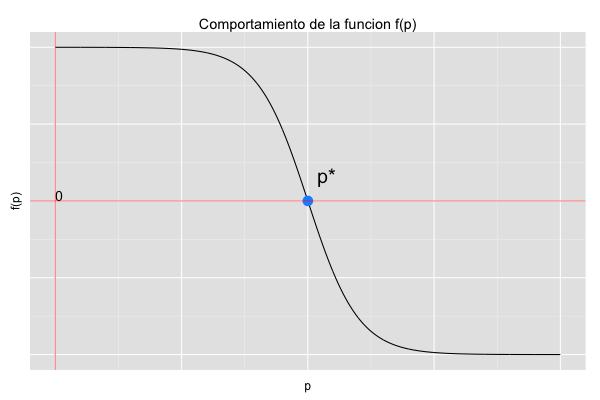
\includegraphics[width=1\textwidth]{Figures/Chapter2_fp}	
%   \caption[Comportamiento de $f(\rho)$.]
%   {La función $f(\rho)$ es no creciente para toda $\rho$. El valor de $f(\rho) = \lambda_{G(\rho)1}+ \lambda_{G(\rho)2} + ... +\lambda_{G(\rho)p}.$ $f(\rho^*) = 0 $}
% \end{figure}
% 
% 
% \begin{example} \label{ex:1}
% Para ejemplificar el lema 1.4 se muestran las matrices $A,B \in {\rm I\!R}^{3 \times 3}$. Para el valor de $f(\rho)$ se utiliza la propiedad (1.29):
% 
% $$f(\rho) = \lambda_{G(\rho)1} + \lambda_{G(\rho)2} + ... + \lambda_{G(\rho)p}$$
% 
% con $p$ la dimensión a la que se va a proyectar. 
% 
% 
% \begin{equation*}
% A = \left(\!
%     \begin{array}{ccc}
%       4 & 0 & 0 \\
%       0 & 6 & 0 \\
%       0 & 0 & 8 
%     \end{array}
%   \!\right), \quad
% B = \left(\!
%     \begin{array}{ccc}
%       1.5 & 0 & 0 \\
%       0 & 2.5 & 0 \\
%       0 & 0 & 5 
%     \end{array}
% \!\right) 
% \end{equation*}
% 
% 
% 
% \begin{equation*}
% G(\rho) = A- \rho B = \left(\!
%     \begin{array}{ccc}
%       4-1.5\rho & 0 & 0 \\
%       0 & 6-2.5\rho & 0 \\
%       0 & 0 & 8-5\rho 
%     \end{array}   	
%       \!\right) 
% \end{equation*}
% 
% Los eigenvalores de esta matriz son $4-1.5\rho$,  $6-2.5\rho$ y  $8-5\rho$. Las funciones graficadas de estos eigenvalores se presentan en la figura 1.5.
% 
% \begin{figure}[!ht] \label{Fig1.4}
%   \centering
%   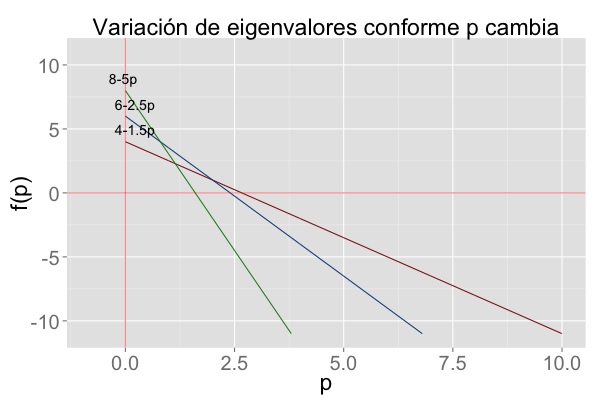
\includegraphics[width=1\textwidth]{Figures/Chapter2_3eigen}  
%   \caption[Gráfica de los eigenvalores en función de $\rho$.] {Cada línea representa como se comporta cada eigenvalor de $A- \rho B$ cuando se varía $\rho$.}
% \end{figure}
% 
% Cuando se desea que el proyector sea de dimensión 1, entonces se tiene que $f(\rho)$ es el eigenvalor más grande,  cuando sea de dimensión 2, la suma de los dos más grandes y así respectivamente. El valor de $f(\rho)$ para estos tres casos está representado en la figura 1.5.
% 
% \begin{figure}[!ht] \label{Fig1.5}
%   \centering
%   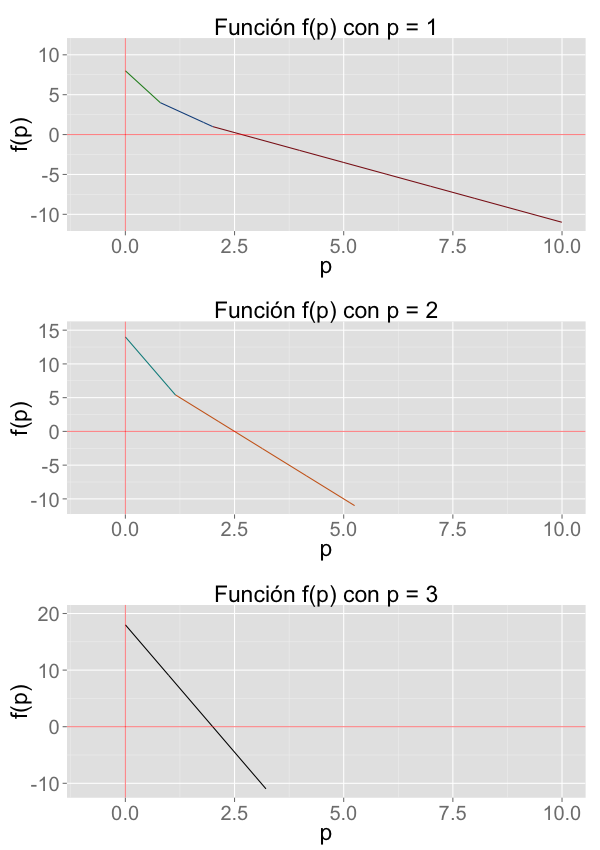
\includegraphics[width=1\textwidth]{Figures/Chapter2_grid3eigen}  
%   \caption[$f(\rho)$ para proyectores de 1,2 y 3 dimensiones.] {La figura superior representa a $f(\rho) = \lambda_{G(\rho)_1}$, la de enmedio $f(\rho) = \lambda_{G(\rho)_1} + \lambda_{G(\rho)_2}$ y la de abajo $f(\rho) = \lambda_{G(\rho)_1} + \lambda_{G(\rho)_2} + \lambda_{G(\rho)_3}$.}
% \end{figure}
% 
% \end{example}
% \pagebreak
% 
% \subsection{Localización del óptimo}
% 
% En la sección anterior se encontró que la maximización al cociente de trazas puede ser visto como el problema de encontrar la raíz de la función $f(\rho) = max_{V^T V= I} \Tr(V^T(A-\rho B)V)$. Por esto, encontrar un intervalo $(\rho_1, \rho_2)$ que contenga al valor óptimo $\rho^*$ puede reducir el número de iteraciones del método. Usando el lema 1.4 se sabe que $f$ es una función no creciente de $\rho$. Por esta razón si se encuentra una $\rho_1$ y $\rho_2$ tal que $f(\rho_1) \geq 0$ y $f(\rho_2) \leq 0$ y con la propiedad de continuidad de la funcion $f(\rho)$ entonces se encontró un intervalo que contiene a $\rho^*$. 
% 
% En esta tesis se dan cotas para el valor de $\rho^*$, la primera en función los eigenvalores de una transformación de $B -\rho A$ y la segunda en función de los eigenvalores de $B$ y $A$ \cite{ngo2012trace}. La demostración de cada una requiere del conocimiento del concepto de inercia y del Teorema de la Inercia de Sylvester. Por este motivo se presentan a continuación: \footnote{La demostración de este teorema puede ser encontrada en \cite{golub2012matrix}.}
% 
% \begin{definition}
% La inercia de una matriz simétrica $A$ es la tripleta de enteros no negativos $(m, z, p)$ donde $m$, $z$ y $p$ son respectivamente el número de eigenvalores negativos, cero y positivos de $A$ \cite{golub2012matrix}.
% \end{definition}
% 
% \begin{theorem}\label{teorem.2}
% Sea $A \in {\rm I\!R}^{n \times n}$ una matriz simétrica y $Z \in {\rm I\!R}^{n \times n}$ no singular. Entonces $A$ y $Z^T A Z$ tienen la misma inercia \cite{golub2012matrix}.
% \end{theorem}
% 
% \begin{proposition}
% La raíz $\rho^*$ de $f(\rho)$ está localizada en el intervalo $(\lambda_p, \lambda_1)$ donde $\lambda_p$ es el p-ésimo eigenvalor más grande de $Z^T(A-\rho B)Z$.
% \end{proposition}
% 
% \begin{proof}
% Sea $Z$ la matriz que diagonaliza a $A-\rho B$ de manera que\footnote{El cálculo de esta matriz puede obtenerse en el algoritmo 8.7.1 de \cite{golub2012matrix}}:
% 
% \begin{equation}\label{eq:2.38}
% \begin{aligned}
%  Z^T AZ = \Lambda \\ Z^T B Z = I
%  \end{aligned}
% \end{equation}
% 
% Con $\Lambda$ una matriz diagonal y $\mu_1, \ldots,  \mu_n$ sus respectivos eigenvalores e $I$ la identidad de tamaño $n$. Entonces por el teorema 1.2 se sabe que $A- \rho B$ y $Z^T(A- \rho B)Z = \Lambda -\rho I$ tienen el mismo número de eigenvalores positivos, negativos y cero. Por lo tanto, la matriz en cuestión es de la siguiente forma:
% 
% \begin{equation}\label{eq:2.39}
% \Lambda - \rho I = 
% \left(\!
%     \begin{array}{cccc}
%       \mu_1 & 0 & \hdots & 0\\
%       0 & \mu_2 & \hdots & 0\\
%       \vdots & \vdots & \ddots & \vdots \\
%       0 & 0 & \hdots & \mu_n
%     \end{array}
%   \!\right) - \rho
%   \left(\!
%     \begin{array}{cccc}
%       1 & 0 & \hdots & 0\\
%       0 & 1 & \hdots & 0\\
%       \vdots & \vdots & \ddots & \vdots \\
%       0 & 0 & \hdots & 1
%     \end{array}
%   \!\right) 
% \end{equation} 
% 
% Como la  matriz $V$ de (1.9) es de tamaño $n \times p$, solo nos interesa saber el signo de los $p$ eigenvalores más grandes. Tomando $\rho = \mu_p$ entonces los elementos de la diagonal de la matriz $\Lambda- \rho I$ son de la forma:
% 
% 
% \begin{equation}\label{eq:2.40}
% \begin{aligned}
%    \mu_i - \mu_p & \geq 0  \quad para \quad i \geq p\\
%    \mu_i - \mu_p & \leq 0  \quad para \quad i \leq p
% \end{aligned}
% \end{equation} 
% 
% Los primeros p elementos tienen la propiedad de ser no negativos, ya que $\lambda_{(A-\rho B)_1} \geq \lambda_{(A-\rho B)_2} \geq ... \geq \lambda_{(A-\rho B)_p}$. Usando el teorema 1.2 se sabe que los primeros p eigenvalores de $A-\rho B$ también son no negativos. Por ende la suma de ellos es mayor o igual que cero. 
% 
% Por otro lado si se toma $\rho = \mu_1$. Entonces los elementos de la diagonal de la matriz (1.38) son de la forma:
% 
% \begin{equation}\label{eq:2.41}
%    \mu_i - \mu_1  \leq 0 \quad \forall \quad i
% \end{equation} 
% 
% Con $i = 1, ..., p$, cada uno de los elementos de la diagonal tiene la propiedad de ser no positivo por el mismo argumento que el caso pasado. Por lo tanto los $p$ eigenvalores más grandes de $\Lambda - \rho I$ y de $A-\rho B$ son no positivos, por lo que su suma es menor o igual que cero:
% 
% \begin{equation}\label{eq:2.42}
%   \rho = \mu_p  \Rightarrow \sum_{i=1}^{p} (\mu_i- \mu_p) \geq 0 \Rightarrow f(\rho) \geq 0
% \end{equation}
% 
% \begin{equation}\label{eq:2.43}
%   \rho = \mu_1  \Rightarrow \sum_{i=1}^{p} (\mu_i - \mu_1) \leq 0 \Rightarrow f(\rho) \leq 0
% \end{equation}
% 
% \end{proof}
% 
% \pagebreak
% 
% \begin{example} \label{ex:2}
% Tomando las matrices A,B iguales que en el ejercicio 1.1, se puede encontrar fácilmente a la matriz $Z$:
% 
% 
% \begin{equation*}
% Z = \left(\!
%     \begin{array}{ccc}
%       \sqrt(\frac{1}{1.5}) & 0 & 0 \\
%       0 & \sqrt(\frac{1}{2.5}) & 0 \\
%       0 & 0 & \sqrt(\frac{1}{5}) 
%     \end{array}
%   \!\right)
% \end{equation*}
% 
% Con la matriz $Z$ definida de esta manera, $Z^T A  Z = \Lambda$ y $Z^T B Z = I$ toman la siguiente forma:
% 
% \begin{equation*}
% \Lambda - \rho I = 
% \left(\!
%     \begin{array}{ccc}
%       \frac{4}{1.5} & 0  & 0\\
%       0 & \frac{6}{2.5}  & 0\\
%       0 & 0 & \frac{8}{5}
%     \end{array}
%   \!\right) - \rho
%   \left(\!
%     \begin{array}{ccc}
%       1 & 0 & 0\\
%       0 & 1 & 0\\
%       0 & 0 & 1
%     \end{array}
%   \!\right) 
% \end{equation*}
% 
% Entonces se puede encontrar un intervalo tal que $\rho^* \in \big[\rho_1, \rho_2 \big]$:
% 
% \begin{equation*}
%   \begin{aligned}
% \rho_1 &= \mu_p \\
% \rho_2 &= \mu_1  
%   \end{aligned}
% \end{equation*}
% 
% Conforme el tamaño de la dimensión a proyectar cambia, las cotas son las siguientes:
% 
% \begin{equation*}
%   \begin{aligned}
%   p =& 1 \Rightarrow \qquad \rho_1 = \frac{4}{1.5} \quad y \quad \rho_2 = \frac{4}{1.5}\\
%   p =& 2 \Rightarrow \qquad \rho_1 = \frac{4}{1.5} \quad y \quad \rho_2 = \frac{6}{2.5} \\
%   p =& 3 \Rightarrow \qquad \rho_1 = \frac{4}{1.5} \quad y \quad \rho_2 = \frac{8}{5}
%   \end{aligned}
% \end{equation*}
%  
% 
%  Estas cotas se pueden ver más fácil en la figura 1.6,donde se observa $f(\rho)$ con respecto a $p$:
% 
% \begin{figure}[!ht] \label{Fig1.6}
%   \centering
%   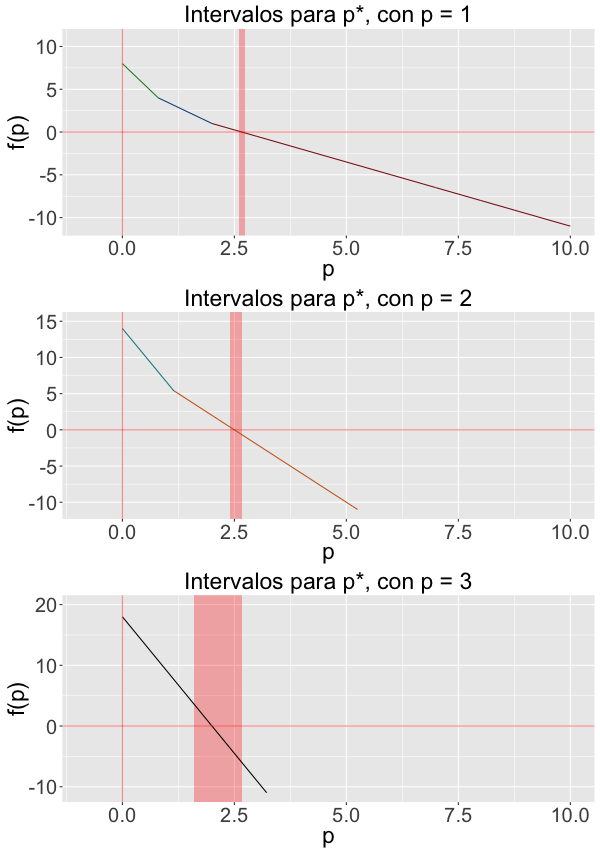
\includegraphics[width=.9\textwidth]{Figures/Chapter2_grid3eigen_interv}  
%   \caption[Intervalos para $\rho^*$. (Primera cota)] {La figura superior representa intervalos para $\rho^*$ cuando $f(\rho) = \lambda_{G(\rho)_1}$, la de enmedio cuando $f(\rho) = \lambda_{G(\rho)_1} + \lambda_{G(\rho)_2}$ y la de abajo cuando $f(\rho) = \lambda_{G(\rho)_1} + \lambda_{G(\rho)_2} + \lambda_{G(\rho)_3}$.}
% \end{figure}
% 
% \end{example}
% 
% Otro intervalo que se ha desarrollado tiene que ver con directamente con los eigenvalores de $A$ y $B$ en lugar de los obtenidos por la matriz $A-\rho B$:
% 
% \pagebreak
% \begin{proposition}
% Sea $B$ positiva definida, entonces la raíz $\rho^*$ de $f(\rho)$ es tal que \cite{ngo2012trace}:
% 
% \begin{equation*}
% \frac{\sum_{i = 1}^{p}\lambda_{A_i}}{\sum_{i = 1}^{p}\lambda_{B_i}} \leq \rho^* \leq \frac{\sum_{i = 1}^{p}\lambda_{(A)_i}}{\sum_{i = 1}^{p}\lambda_{(B)_{n-i+1}}}	
% \end{equation*}
% 
% con $\lambda_{A_i}$ y $\lambda_{B_i}$ el i-ésimo eigenvalor más grande  de la matriz $A$ y $B$ respectivamente \cite{ngo2012trace}. 
% \end{proposition}
% 
% 
% \begin{proof}
% Se tiene la propiedad que para una $p$ dada:
% 
% 
% \begin{equation}\label{eq:2.44}
% \max_{V^T V = I} \Tr(V^T A V) =  \Tr(V^{T*} A V^*) = \sum_{i=1}^p \lambda_{A_i }
% \end{equation}
%  
% Con $\lambda_{A_i}$ los eigenvalores de A. Como esta $V^*$ maximiza la traza sobre $A$, entonces no necesariamente maximiza la de $B$. Al sustituirla en $\Tr(V^{T} B V)$ se tiene que: 
% 
% \begin{equation}\label{eq:2.45}
% \Tr(V^{T*} B V^*) \leq \sum_{i=1}^p \lambda_{B_i }
% \end{equation}
% 
% Con $\lambda_{B_i}$ los eigenvalores de B. Al hacer el cociente de (1.43) y (1.44) Se puede acotar inferiormente a $\rho^*$:
% 
% 
% \begin{equation*}
%   \frac{\sum_{i=1}^p \lambda_{A_i}} {\sum_{i=1}^p \lambda_{B_i}} \leq \frac{\Tr(V^{T*} A V^*)}{\Tr(V^{T*} B V^*)} \leq \max_{V^T V} \frac{\Tr(V^{T} A V)}{\Tr(V^{T} B V)} = \rho^*
% \end{equation*}
% 
% Ahora falta acotarlo superiormente. Usando las siguientes propiedades que son derivadas de (1.27):
% 
% \begin{equation}\label{eq:2.46}
%   \Tr(V^T A V) \leq \sum_{i=1}^p \lambda_{A_i} 
% \end{equation}
% 
% \begin{equation}\label{eq:2.47}
%   \Tr(V^T B V) \geq \sum_{i=1}^p \lambda_{B_{(n-i+1)}}
% \end{equation}
% 
% La expresión (1.46) es la suma de los p eigenvalores más chicos de $B$. Dividiendo (1.45) entre (1.46) se tiene que para cualquier matriz ortogonal $V$:
% 
% \begin{equation}\label{eq:2.48}
%    \frac{\Tr(V^{T} A V)}{\Tr(V^{T} B V)} \leq \frac{\sum_{i=1}^p \lambda_{A_i}}{\sum_{i=1}^p \lambda_{B_{(n-i+1)}}}
% \end{equation}
% 
% En particular si se toma $V = V^{**}$ (La matriz con la que se alcanza $\rho^*)$:
% 
% \begin{equation}\label{eq:2.49}
%   \rho^* = \frac{\Tr(V^{T**} A V^{**})}{\Tr(V^{T**} B V^{**})} \leq \frac{\sum_{i=1}^p \lambda_{A_i}}{\sum_{i=1}^p \lambda_{B_{(n-i+1)}}}
% \end{equation}
% 
% \end{proof}
% \begin{example}
% Para ejemplificar esta cota se usará las matrices $A$ y $B$ de los dos ejemplos anteriores y se muestra en la figura 1.7.
% 
% 
% \begin{equation*}
% A = \left(\!
%     \begin{array}{ccc}
%       4 & 0 & 0 \\
%       0 & 6 & 0 \\
%       0 & 0 & 8 
%     \end{array}
%   \!\right), \quad
% B = \left(\!
%     \begin{array}{ccc}
%       1.5 & 0 & 0 \\
%       0 & 2.5 & 0 \\
%       0 & 0 & 5 
%     \end{array}
% \!\right) 
% \end{equation*}
% 
% 
% (i) Para $p = 1$ la cota es la siguiente:
% \begin{equation*}
% \begin{aligned}
%   \lambda_{A_1} = 8 \qquad
%   \lambda_{B_1} = 5 \qquad
%   \lambda_{B_3} = 1.5
% \end{aligned}
% \end{equation*}
% 
% \begin{equation*}
% \begin{aligned}
% \rho_1 = \frac{\sum_{i = 1}^{p}\lambda_{A_i}}{\sum_{i = 1}^{p}\lambda_{B_i}}  = \frac{8}{5} \qquad
% \rho_2 = \frac{\sum_{i = 1}^{p}\lambda_{A_i}}{\sum_{i = 1}^{p}\lambda_{B_{n-i+1}}}  = \frac{8}{1.5}
% \end{aligned}
% \end{equation*}
% 
% (ii) Para $p = 2$ la cota es la siguiente:
% 
% \begin{equation*}
% \begin{aligned}
% \sum_{i = 1}^{2}\lambda_{A_1}  =& 14 \qquad
% \sum_{i = 1}^{2}\lambda_{B_1}  =& 7.5 \qquad
% \sum_{i = 1}^{2}\lambda_{B_{3-i+1}} =& 4
% \end{aligned}
% \end{equation*}
% 
% \begin{equation*}
% \begin{aligned}
% \rho_1 = \frac{\sum_{i = 1}^{p}\lambda_{A_i}}{\sum_{i = 1}^{p}\lambda_({B_i)}}
%  = \frac{14}{7.5} \qquad
% \rho_2 = \frac{\sum_{i = 1}^{p}\lambda_{A_i}}{\sum_{i = 1}^{p}\lambda_{B_{n-i+1}}}  = \frac{14}{4}
% \end{aligned}
% \end{equation*}
% 
% 
% 
% (iii) Para $p = 3$ la cota es la siguiente:
% \begin{equation*}
%   \begin{aligned}
%   \sum_{i = 1}^{3}\lambda_{A_1}  = 18 \qquad
%   \sum_{i = 1}^{3}\lambda_{B_1}  = 9 \qquad
%   \sum_{i = 1}^{3}\lambda_{B_{n-i+1}}  = 9
%   \end{aligned}
% \end{equation*}
% 
% \begin{equation*}
%   \begin{aligned}
% \rho_1 = \frac{\sum_{i = 1}^{p}\lambda_{A_i}}{\sum_{i = 1}^{p}\lambda_{B_i}}  = \frac{18}{9} \qquad
% \rho_2 = \frac{\sum_{i = 1}^{p}\lambda_{A_i}}{\sum_{i = 1}^{p}\lambda_{B_{n-i+1}}}  = \frac{18}{9}
%   \end{aligned}
% \end{equation*}
% 
% \end{example}
% 
% \begin{figure}[!ht] \label{Fig1.7}
%   \centering
%   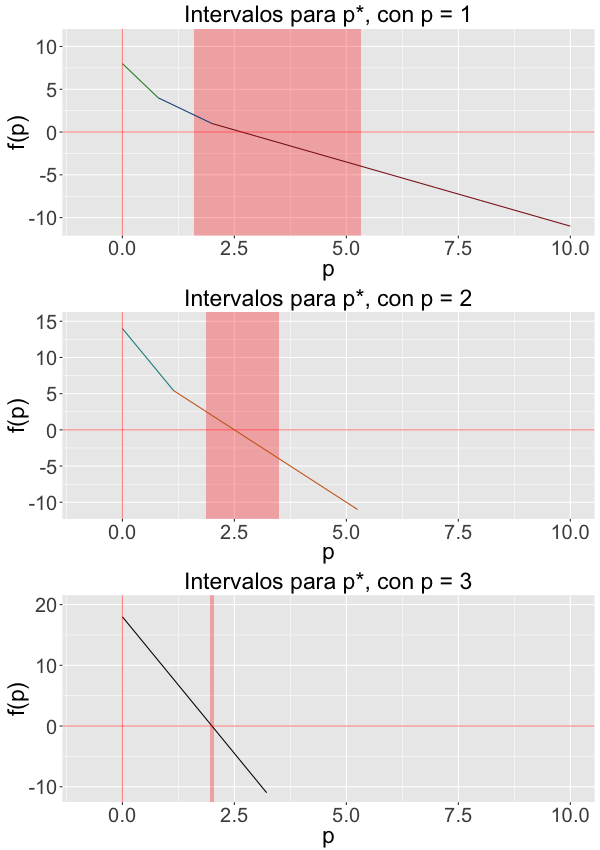
\includegraphics[width=.9 \textwidth]{Figures/Chapter2_grid3eigen_interv2}  
%   \caption[Intervalos para $\rho^*$. (Segunda cota)] {La figura superior representa intervalos para $\rho^*$ cuando $f(\rho) = \lambda_{G(\rho)_1}$, la de enmedio cuando $f(\rho) = \lambda_{G(\rho)_1} + \lambda_{G(\rho)_2}$ y la de abajo cuando $f(\rho) = \lambda_{G(\rho)_1} + \lambda_{G(\rho)_2} + \lambda_{G(\rho)_3}$.}
% \end{figure}
% 
% 
% 
